\documentclass[a4paper,11pt]{article}

\usepackage[empty]{fullpage}
\usepackage{titlesec}
\usepackage[usenames,dvipsnames]{color}
\usepackage{enumitem}
\usepackage{fancyhdr}
\usepackage[english]{babel}
\usepackage{tabularx}
\usepackage{fontawesome5}
\usepackage{multicol}
\usepackage{graphicx}
\usepackage[export]{adjustbox}
\usepackage[sfdefault]{roboto}
\usepackage[hidelinks]{hyperref}
\usepackage{montserrat}

\setlength{\multicolsep}{3.0pt}
\setlength{\columnsep}{5pt}

% Adjust footer
\pagestyle{fancy}
\fancyhf{} % clear all header and footer fields
\renewcommand{\headrulewidth}{0pt}
\renewcommand{\footrulewidth}{0pt}
\setlength{\footskip}{5pt} % Increase footskip to resolve fancyhdr warning

% Adjust margins
\addtolength{\oddsidemargin}{-0.5in}
\addtolength{\evensidemargin}{-0.5in}
\addtolength{\textwidth}{1.0in}
\addtolength{\topmargin}{-.7in}
\addtolength{\textheight}{1.3in}

\urlstyle{same}

\raggedbottom
\raggedright
\setlength{\tabcolsep}{0in}

% Sections formatting
\titleformat{\section}{
  \vspace{-6pt}\scshape\raggedright\large\bfseries
}{}{0em}{}[\color{black}\titlerule \vspace{-7pt}]

% Ensure that generate pdf is machine readable/ATS parsable
\pdfgentounicode=1

% Custom commands
\newcommand{\resumeItem}[1]{
  \item\small{#1 \vspace{-2pt}}
}

\newcommand{\resumeSubheading}[4]{
  \vspace{-2pt}\item
    \begin{tabular*}{0.97\textwidth}[t]{l@{\extracolsep{\fill}}r}
      \textbf{#1} & \textbf{\small #2} \\
      \textit{\small#3} & \textit{\small #4} \\
    \end{tabular*}\vspace{-7pt}
}

\newcommand{\resumeProjectHeading}[2]{
    \item
    \begin{tabular*}{0.97\textwidth}{l@{\extracolsep{\fill}}r}
      \small#1 & \textbf{\small #2} \\
    \end{tabular*}\vspace{-7pt}
}

\newcommand{\resumeSubHeadingListStart}{\begin{itemize}[leftmargin=0.15in, label={}]}
\newcommand{\resumeSubHeadingListEnd}{\end{itemize}}
\newcommand{\resumeItemListStart}{\begin{itemize}}
\newcommand{\resumeItemListEnd}{\end{itemize}\vspace{-5pt}}

\begin{document}
	
	\begin{minipage}[c]{0.15\textwidth}
		\fbox{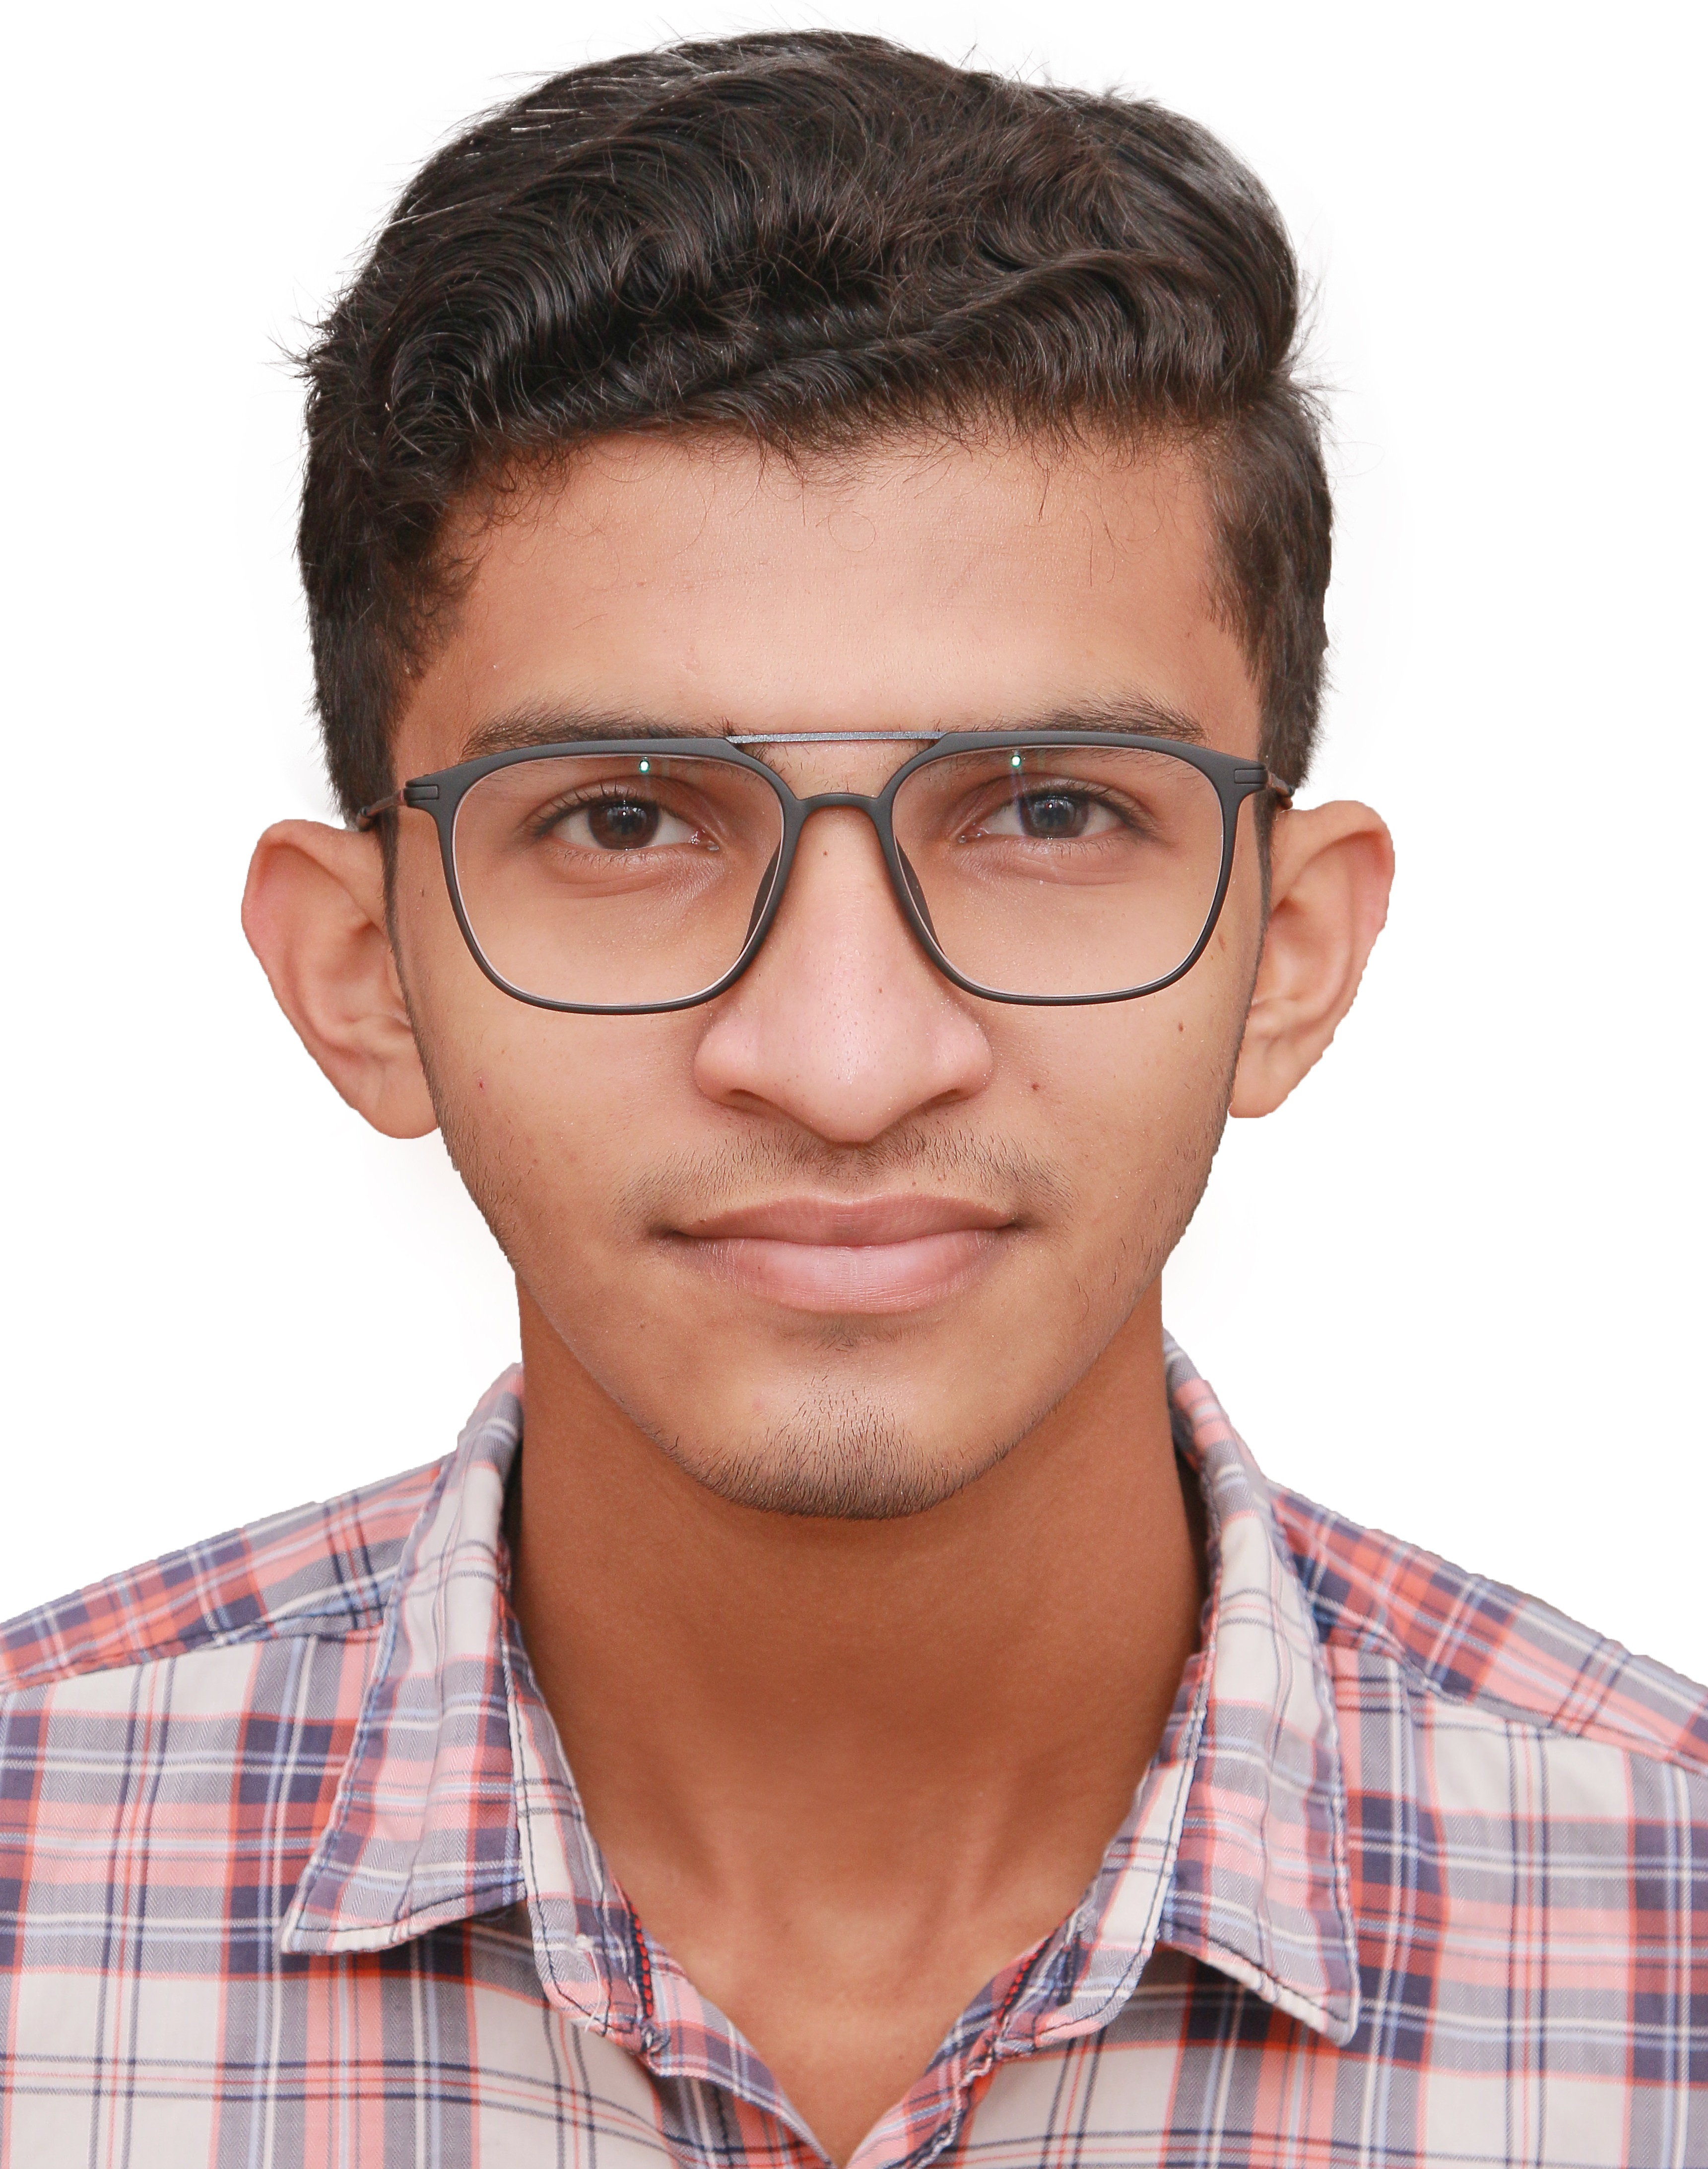
\includegraphics[width=0.84\textwidth]{photo.jpg}}  
	\end{minipage}
	\begin{minipage}[t]{0.84\textwidth}  % Increased from 0.7 to 0.8 to use remaining space
		\begin{center}
			{\fontfamily{Montserrat-TOsF}\selectfont \textbf{ \Huge \scshape Ajmal Basheer}} \\ \vspace{1pt}
			\small{
				\raisebox{-0.1\height}\faPhone\ \href{tel:+919496444520}{\underline{+91 9496444520}} $|$ 
				\raisebox{-0.2\height}\faEnvelope\ \href{mailto:ajmalbuv@gmail.com}{\underline{ajmalbuv@gmail.com}} $|$ 
				\raisebox{-0.2\height}\faLinkedin\ \href{https://linkedin.com/in/ajmalbuv}{\underline{linkedin.com/ajmalbuv}} $|$
				\raisebox{-0.2\height}\faGithub\ \href{https://github.com/ajmalbuv}{\underline{github.com/ajmalbuv}}
			}
		\end{center}
	\end{minipage}

\section{Summary}
\begin{itemize}[leftmargin=0.15in, label={}]
  \small{\item{
        Driven Computer Applications student with hands-on experience across full-stack development, Deployment, and Maintenance. Skilled in Python, Django, and PostgreSQL, with a firm understanding of creating scalable applications, streamlining operations, and optimizing system performance. Adaptable and eager to contribute to innovative solutions and uphold high-quality standards in dynamic IT environments.
        }}
\end{itemize}
\section{Education}
\resumeSubHeadingListStart
\resumeSubheading
{Krupanidhi Degree College}{Bengaluru, Karnataka}
{Bachelor of Computer Applications}{Aug. 2021 -- July 2024}
\resumeSubheading
{MIC Higher Secondary School}{Malappuram, Kerala}
{Commerce}{June 2017 -- March 2019}
%  \resumeSubheading {International Indian School Dammam}{Dammam, Saudi Arabia}{CBSE}{March 2017}
\resumeSubHeadingListEnd

%\section{Relevant Coursework}
%\begin{itemize}[leftmargin=*,nosep]
%  \begin{multicols}{4}
%    \item Computer Networks
%    \item Operating Systems
%    \item Database Management% Systems
%    \item Web Development
%    \item Data Structures% and Algorithms
%    \item Cyber Security
%    \item Software Engineering
%    \item Cloud Computing
%  \end{multicols}
%\end{itemize}

\section{Core Competencies}
\begin{itemize}[leftmargin=*,nosep]
	\begin{multicols}{3}
		\item Full Stack Development
		\item System Optimization 
		\item API Development
		\item Cloud Deployment
		\item Troubleshooting and Debugging
		\item Quality Assurance and Testing
	\end{multicols}
\end{itemize}

\section{Experience}
\resumeSubHeadingListStart
\resumeSubheading
{WIMD Technologies Pvt Ltd}{May 2024 -- June 2024}
{Software Engineer Intern}{Bengaluru, Karnataka}
\resumeItemListStart
\resumeItem{Completed a full-time, ten-day internship with \textbf{WIMD Technologies Pvt Ltd}, immersing in real-world scenarios and working on industry-standard tools to complement my academic learning.}
\resumeItem{\textbf{Developed and Optimized APIs:} Successfully created RESTful APIs using Node.js, implementing secure authentication (JWT) and role-based authorization for data integration between applications, ensuring adherence to industry best practices.}
\resumeItem{\textbf{Database Design and Performance:} Assisted in designing, maintaining, and optimizing MongoDB databases, including schema creation and indexing, which enhanced data retrieval speed and ensured high performance for large datasets.}
\resumeItem{\textbf{API Testing and Quality Assurance:} Utilized Postman to develop and execute automated test scripts, identifying and troubleshooting issues across GET, POST, PUT, and DELETE requests, ensuring reliable API performance.}
\resumeItem{\textbf{Collaborative Problem Solving:} Engaged in team-based debugging and code review sessions, leveraging critical thinking and communication skills to resolve database connectivity and API integration challenges efficiently.}
\resumeItemListEnd
\resumeSubHeadingListEnd

\section{Projects}
\resumeSubHeadingListStart
\resumeProjectHeading
{\textbf{\href{https://github.com/ajmalbuv/EduManage}{\underline{EduManage}}} $|$ \emph{Python, Django, PostgreSQL, Docker}}{July 2024}
\resumeItemListStart
\resumeItem{\textbf{Developed and Deployed Scalable Web Application:} Built an end-to-end web application using Django and PostgreSQL, enhancing data management and administrative efficiency for users.}
\resumeItem{\textbf{Cross-Platform Deployment for High Availability:} Implemented on an Ubuntu VPS with Gunicorn and Certbot for SSL, as well as Vercel using serverless functions, ensuring 99\%+ uptime.}
\resumeItem{\textbf{Optimized Database and Security:} Designed efficient database schemas and deployed SSL encryption to secure user data, achieving a 30\% improvement in query performance.}
\resumeItem{\textbf{Collaborative Version Control:} Leveraged GitHub for collaborative development, enhancing workflow efficiency and documentation for seamless project management.}
\resumeItemListEnd
\resumeSubHeadingListEnd

\section{Technical Skills}
\begin{itemize}[leftmargin=0.15in, label={}]
	\small{\item{
			\textbf{Programming Languages}{: Python, Java, JavaScript, SQL, C, PHP, Dart, R}\\
			\textbf{Web Technologies}{: HTML5, CSS3, React.js, Node.js, Django, Flask, REST APIs, Flutter}\\
			\textbf{Databases \& Tools}{: PostgreSQL, MongoDB, Docker (containers), Git (version control), Oracle Cloud}\\
			\textbf{Development Tools}{: VS Code, PyCharm, IntelliJ, Postman, Android Studio}
	}}
\end{itemize}

\end{document}
